


\chapter{Results}
\label{Sec:physicalOuts}

\section{Device}

The main physical output of this project has of course been the device itself, which has already gone through a few iterations just in this short year.

\subsection{Initial Designs}

The schematic design for the device was done in KiCAD, an open-source electronics design software suite. This was chosen due to familiarity and the flexibility for adding components that are not built in. There are also extensive libraries, including a DigiKey library that adds many of the parts stocked by DigiKey for ease of design.

These designs were then laid out into prototype \acrshort{pcbs} that were ordered through JLCPCB for economical production, including pick-and-place of the surface-mount components. These \acrshort{pcbs} were designed with the USB and LED modules connected to the main board with mouse-bites, to allow for them to be snapped off after testing. This way the prototype board could be conveniently connected to all the required parts for testing, then could be snapped into its component parts for more accurate modelling of the final product. These snappable daughter boards could be reconnected to the main board via pin headers for each of the required connections, meaning they could be mounted directly back on to the main board, or connected via wires at a distance (in a more similar way to how the final product would function). 

\begin{figure}[bt]
\centering
\includegraphics[width=0.45\textwidth]{images/pcb3d1.png}
\caption{3D render of the first set of \acrshort{pcbs} created in KiCAD. Top right is the snappable LED module, the USB programmer is on the bottom right snappable daughter-board.}
\label{Fig:PCB1}
\end{figure}

Unfortunately, due to England's national lockdown, this round of \acrshort{pcbs} could not be retrieved and were returned to JLCPCB. This meant that alternative action had to be taken. Furthermore, due to the University's policy on soldering at home during the lockdown, they would not have been able to be completed either way.

\subsection{Breadboard}

For this reason, an alternative approach was required. A solderless breadboard was acquired and breadboard-friendly components were ordered. A breadboard prototype was then produced from the original schematics, as shown in Figure \ref{Fig:breadboard}.

An ESP32 board was required to ensure that the main function would be the same as the schematics. The Feather Huzzah32 from Adafruit was a board using the same programming chip (CP2104), as well as having the ESP32 and an optional ``wing'' that could add the PCF8523 \acrfull{rtc} and a micro-SD card slot, much the same as that on the schematic.

\begin{figure}[tb]
\centering
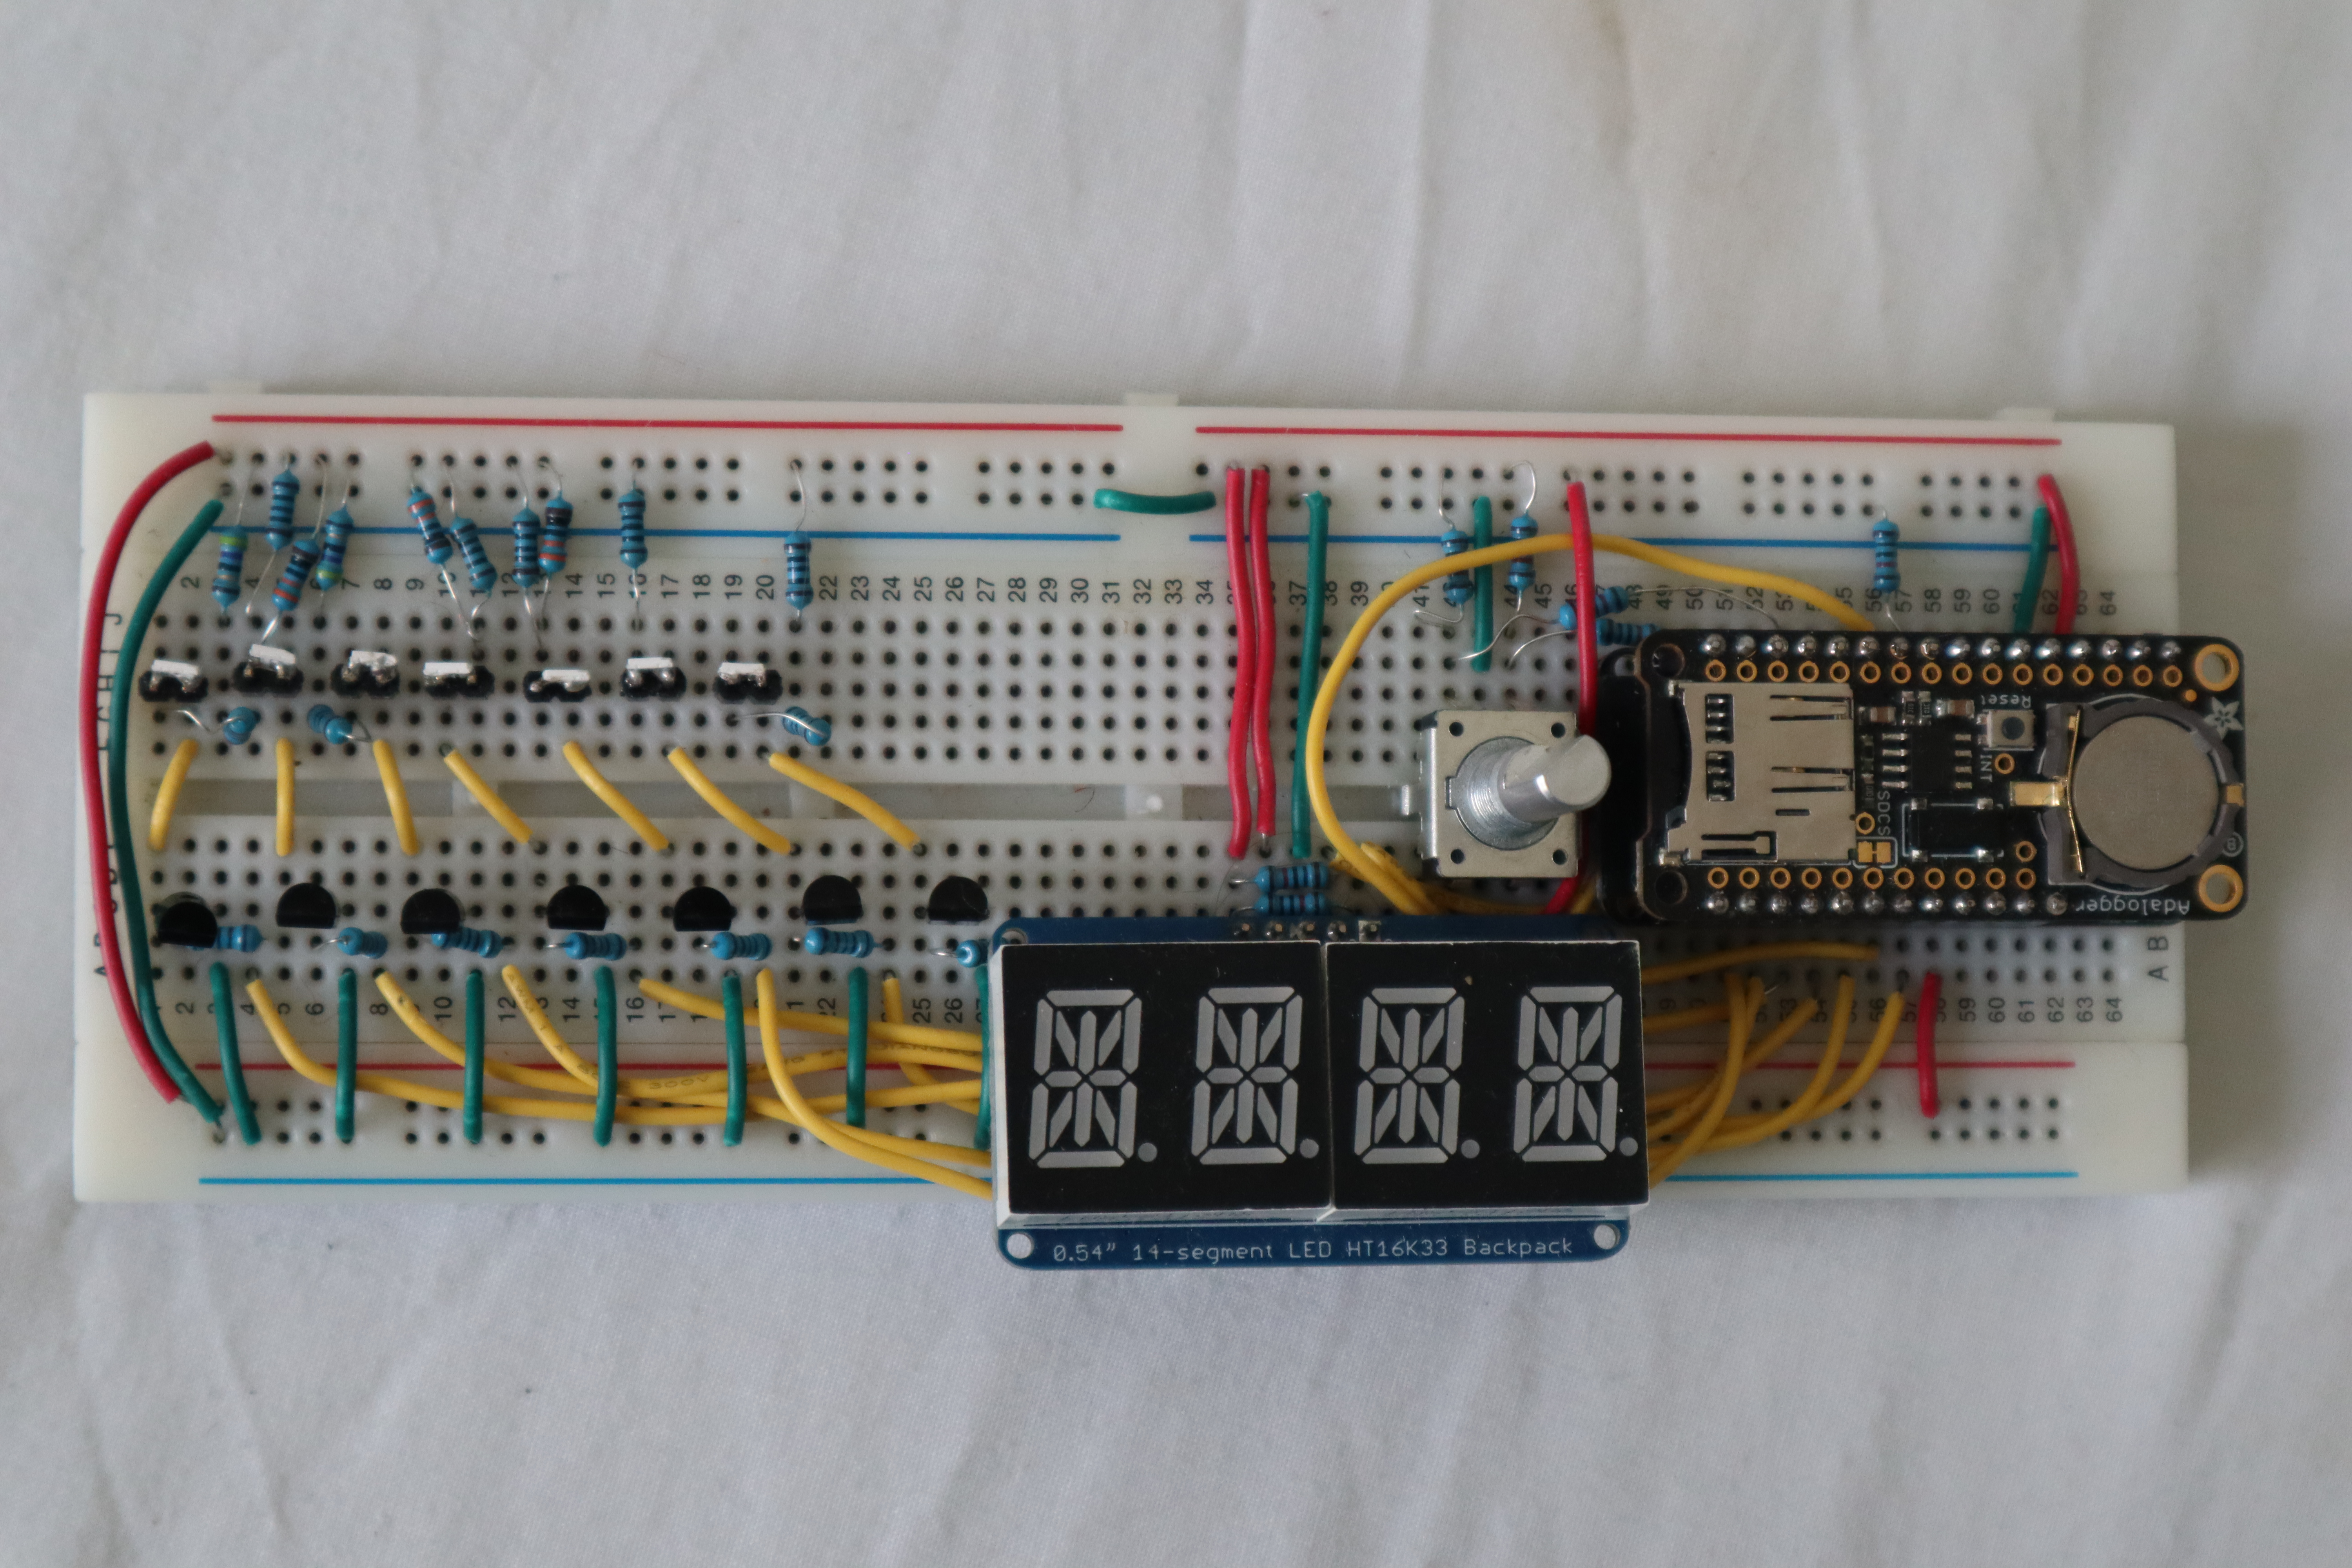
\includegraphics[width=0.45\textwidth]{images/Breadboard.JPG}
\caption{The breadboard prototype used as a proxy for the real device.}
\label{Fig:breadboard}
\end{figure}

The same LEDs were used on the breadboard as were going to be used on the \acrshort{pcbs} so that the outputs would be the same. The other components were kept as similar as possible, with all of the through-hole components remaining the same.

\subsection{Firmware}

The prototype was programmed in the Arduino language as many libraries were available that made reading the encoder, writing to the 14-segment display, and changing the brightness of the LEDs trivial.

\subsection{Final Design}

\begin{figure}[bt]
\centering
\includegraphics[width=0.5\textwidth]{images/Concept.png}
\caption{The concept drawing of what the final controller module could look like, as imagined by a product designer.}
\label{Fig:Concept}
\end{figure}


Once it had been confirmed that the breadboard prototype functioned fully and correctly, a new set of \acrshort{pcbs} were ordered, this time with high confidence of them working. 

The boards contained programming capabilities via a micro-usb, including auto-reset functionality for ease of programming. 2 levels of power regulation were included, the 12V that would be the main input and run the LEDs, as well as a 3.3V regulator to run all of the logic circuitry.

A physical reset button was added to ensure the device could be effectively tested and debugged easily. I2C was used to communicate with the \acrshort{rtc} and the screen, and SPI was used to integrate the SD card.

All \acrshort{ic}s were decoupled with a pair of capacitors, 1nF and 100nF to improve the transient response. All external ports were also protected by 15kV \acrshort{esd} diodes. Bulk capacitors were also used to ensure smooth power supply throughout the board, which itself had 4 layers: signal, ground, power, signal.

LEDs were controlled by low-side NPN transistors to decouple them from the logic circuitry. These were mounted on a separate 2-layer board with a large ground plane on both sides to aid thermal regulation.

Both the schematics and PCB layouts can be viewed in Appendix \ref{App:Electronics}.

A product designer was also employed to create a concept drawing for how the final controller device may look if it were developed into a real product. This is shown in Figure \ref{Fig:Concept}.

\section{Simulator}

Alongside the hardware development was the production of the simulator; created in LabVIEW, it was designed to approximate the spectral output of the device to be used to develop the spectra that would be implemented without having to have constant access to the measurement facilities. The LEDs' outputs were approximated using Gaussian and bell-shaped curves, generated in custom made sub-VIs. Sliders were used for simple LED adjustment and a button allows the user to save the current spectrum as a csv file for processing. The LabVIEW code for the simulator can be viewed in Appendix \ref{App:Sim}.

The simulator was calibrated using actual measured spectral outputs from the device, with each LED output being individually tuned first, then all combinations of LEDs being assessed and validated to ensure the interactions between colours was correct. This ensured that the simulator functioned in the same way as the device in all possible scenarios.

\section{Spectrometer}

\begin{figure}[b]
\centering
\includegraphics[width=0.45\textwidth]{images/CDDVD.jpg}
\caption{Microscope images of a CD and DVD, the DVD has much smaller pits, equating it to a higher resolution diffraction grating \citep{avsdiskcreatorAVS4YOUAVSDisc2019}.}
\label{Fig:CDDVD}
\end{figure}

Measuring the actual device was also made significantly harder due to the lockdown. Access to the hyperspectral camera was revoked in line with the stay-at-home order. An alternative method for recording the spectra had to be found. Many potential solutions were discussed with machine vision specialists, but many of the proposed solutions were not-applicable as they could not capture the entire spectrum.

A spectrometer that could achieve full visible-spectrum range was produced which could be used to gather the spectral data from the device.

This spectrometer was based on a simple slit, that directed light towards a diffraction grating that split the light into its component colours which could be captured with a camera.

For the initial attempt, a box was used with a CD as a diffraction grating and mirror, reflecting the light towards the camera. However, the camera was mounted too far away and could not pick up good images of the spectrum.

The second attempt used a transmissive approach: the mirror-like layer of the CD was removed and the camera could be put directly against it. This time the box was too small, and the slit could be seen in the frame of the image from the camera.

Finally for the third attempt - dubbed $Mk.3$ - a long tube was used as the body, so the camera could not see the slit. 2 Were produced: the reflective ($Mk.3_r$) and transmissive ($Mk.3_t$) models. The diffraction grating was replaced with a DVD to increase the number of lines per millimetre, increasing the detail in the resulting image (See Figure \ref{Fig:CDDVD}).

A Canon M50 DSLR camera with a 15-45mm lens was used to capture the images from the spectrometer. 

\section{Spectral Data}

\begin{figure}[bt]
\centering
	\begin{subfigure}[ht]{0.5\textwidth}
	\includegraphics[width=\textwidth]{images/calibration.png}
	\caption{Spectrum captured of \acrshort{cfl} using the spectrometer}
	\end{subfigure}

	\begin{subfigure}[ht]{0.5\textwidth}
	\includegraphics[width=\textwidth]{images/CFL.jpg}
	\caption{Reference spectrum with labelled peaks \citep{padleckasFileFluorescentLighting2005}}
	\end{subfigure}
	
\caption{Comparison of \acrshort{cfl} spectra. The similarity, even down to the very small peaks (eg. peak 15) shows the impressive accuracy of the spectrometer.}
\label{Fig:CFL}
\end{figure}

\subsection{Spectrometer Validation}

In order to calibrate the readings taken by the spectrometer, a known spectrum with multiple defined peaks must be captured. The peaks can then be labelled, and as the wavelength of each peak is known, a calibration curve can be defined. This equation is then used to scale the x-axis appropriately to show the corresponding wavelengths of all subsequent readings.


\begin{figure}[b]
\centering
\includegraphics[width=0.5\textwidth]{images/CalibrationTracker.png}
\caption{The tracker Physics software being used to extract the spectrum (right) from the spectrometer image (left)}
\label{Fig:process}
\end{figure}


A \acrfull{cfl} was used for this process as the spectrum is clearly defined and contains many distinctive peaks. Figure \ref{Fig:CFL} shows the comparison of the recorded \acrshort{cfl} and a reference spectrum. This validates the accuracy of the spectrometer as these two spectra are remarkably similar. The process of extracting the spectrum from the image using the Tracker Physics software is shown in figure \ref{Fig:process}.

\subsection{Comparing Spectra}

After the spectrometer was validated, the real device data was collected as per the methods set out in chapter \ref{Chap:Meth}. 

\begin{table}[bt]
\centering
\begin{tabular}{l|lll}
          			& Device & HUE    & \acrshort{cfl} \\\hline
\acrfull{morning}   & 0.4954 & 0.6091 & 1.0192 \\
\acrfull{afternoon} & 0.7967 & 1.0138 & 1.1108 \\
\acrfull{evening}   & 0.8226 & 0.9599 & 1.1108 \\
\acrfull{night}     & 1.1688 & 1.0823 & 1.2047
\end{tabular}
\caption{The \acrshort{sam} values corresponding to the lights at different times of day}
\label{Tab:SAM}
\end{table}


\begin{figure}[bt]
\centering
\begin{subfigure}[h]{0.45\textwidth}
	\includegraphics[width=\textwidth]{Images/Spectra/MN.png}
\end{subfigure}
\begin{subfigure}[h]{0.45\textwidth}
	\includegraphics[width=\textwidth]{Images/Spectra/AN.png}
\end{subfigure}

\begin{subfigure}[h]{0.45\textwidth}
	\includegraphics[width=\textwidth]{Images/Spectra/EV.png}
\end{subfigure}
\begin{subfigure}[h]{0.45\textwidth}
	\includegraphics[width=\textwidth]{Images/Spectra/NX.png}
\end{subfigure}
\caption{The 4 spectra at real scale with the melanopsin action spectrum highlighted.}
\label{Fig:Flux}
\end{figure}


\begin{table*}[bt]
\centering
\begin{tabular}{cc|ccccc|c}
 & && &  Lux  && \\
                                &     & Cyanopic & Chloropic & Erythropic & Melanopic & Rhodopic & Phase Shift \\\hline\hline
\multirow{4}{*}{Device}         & \acrshort{morning}  & 2060         & 2390          & 2390           & 2420          & 2390         & 2h38        \\
                                & \acrshort{afternoon}  & 7.83         & 1130          & 1510           & 347           & 612          & 2h23        \\
                                & \acrshort{evening}  & 1.58         & 228           & 494            & 14.8          & 45.8         & 14min       \\
                                & \acrshort{night}  & 0            & 14.4          & 66.5           & 0.09          & 0.69         & 0min        \\\hline
\multirow{4}{*}{\begin{tabular}{c}Philips \\ HUE\end{tabular}}      & \acrshort{morning}  & 1780 		 & 1710 	     & 1700     	  & 1460	      & 1570	     & 2h37        \\
                                & \acrshort{afternoon}  & 1390         & 1700          & 1790           & 1280          & 1460         & 2h36        \\
                                & \acrshort{evening}  & 1090         & 1350          & 1850           & 1120          & 1350         & 2h36        \\
                                & \acrshort{night} & 722          & 1500          & 1760           & 886           & 1130         & 2h35        \\\hline
\multirow{2}{*}{\begin{tabular}{c}Standard \\ Bulbs\end{tabular}} & LED & 78.1         & 94.9          & 97.3           & 81.0          & 87.3         & 1h25        \\
                                & CFL & 66.0         & 95.5          & 97.6           & 82.4          & 86.7         & 1h25        \\
                                & Candle & 0.98		 & 2.95			 & 4.15 		  & 1.57		  & 1.93		 & 0min
\end{tabular}
\caption{$\alpha$-opic equivalent illuminance: how much each photo-pigment is activated by the light from the given sources. }
\label{Tab:Lux}
\end{table*}


As shown in Table \ref{Tab:SAM}, the device consistently performs more closely to the given spectrum (with the exception of the \acrshort{night} condition due to the steepness of the curve of the device). 

Figure \ref{Fig:Spectra} (Appendix \ref{App:Comp}), in which the spectra of the device, the reference spectrum, and those of the Philips HUE and a regular LED are overlaid, backs up these findings. It can clearly be seen that the LED and Philips HUE contain many more frequencies not contained by the reference spectrum from the sun (or fire in the case of the \acrshort{night} condition). This is done in order to approximate the colour with the limited resources available, whereas the natural-lighting device approximates the colour through the approximation of the spectrum.

Figure \ref{Fig:Flux} shows the 4 spectra on the same scale axes, with the y-scale reaching $5.93\mu Wcm^{-2}nm^{-1}$. The colour represents the \acrfull{cct} which for the 4 conditions were 5197k, 2353k, 1107k and 606k respectively. The action spectrum of melatonin is also highlighted and the activation of melanopsin is overlaid on this.


\subsection{Light Quality}

In the \acrshort{morning} condition, the \acrshort{cri} of the device was measured at 92.6 (out of 100) , which is considered artist quality, but obviously decreased through the other conditions: 66.8, 52.1 and 63.4 for \acrshort{afternoon}, \acrshort{evening}, \acrshort{night} respectively.

This high \acrshort{cri} shows the usefulness of this light for working during the day. Even artists and designers who need extremely accurate colour rendering would be able to use this light with faith that it is showing them the true colours.
 
The \acrshort{cfl} and LED received scores of 83.9 and 63.9 respectively. This is because of the lack of certain wavelengths; when the light is reflected from a coloured surface, if that colour's wavelength is absent (eg. cyan in the LED), then the colour will look incorrect. The candle received a \acrshort{cri} of 94.3, despite containing very few short wavelengths. This is an interesting consideration for further study; how could this be achieved with an artificial light?

\section{Circadian Effects}
\label{Sec:CircEffects}

Table \ref{Tab:Lux} shows how much each condition affects the circadian rhythm through the 5 photo-pigments in the eye. The melanopic lux is the most important factor of this calculation, followed by the cyanopic lux. The other photopigments have much smaller neurophysiological effects.

The last column of Table \ref{Tab:Lux} shows the phase shift, which is how much one's circadian rhythm would shift when using this light, so a phase shift of 1h34 means, when using this light, your melatonin secretion is inhibited for 1h34 minutes after use.

From this table it can be seen that the device outperforms all of the other lamps that were tested. The produced device was brighter during the day than any of the other tested devices, but also had a smaller impact before sleep than anything but the candle (both had no effect), although the device, despite having no effect on sleep, was brighter than the candle in the chloropic and erythropic lux catagories, meaning it would be more effective at illuminating a space.

These results show that the device could be used in \acrshort{morning} mode until no less than 2 hours and 40 minutes before sleep onset; \acrshort{afternoon} mode can be used until 2 hours and 25 minutes before sleep. This shows that perhaps in order to prevent an excessively fast change in \acrshort{cct}, \acrshort{morning} mode should transition to \acrshort{afternoon} mode earlier, around 3 - 3.5 hours before sleep. 2.5 hours before sleep, \acrshort{evening} mode should be initiated, which is appropriate up until the last 15 minutes before sleep onset, when \acrshort{night} mode can be employed. This will maximise the amount of the day spent in high \acrshort{cri} lighting, with a period for winding down (\acrshort{afternoon} mode) before moving into the pre-sleep lighting, with \acrshort{evening} mode. in this period, highly visual activities will become more difficult, but reading, puzzles, etc. will still be easily doable. Once \acrshort{night} mode is active, reading will still be possible, but many other activities will not, so this should be only used just before sleep (15 minutes).

